%%%%%%%%%%%%%%%%%%%%%%%%%%%%%%%%%%%%%%%%%%%%%%%%%%%%%%%%%%%%%%%%%%%%%%%%%%
%%%%%%%%%%%%   CAPTER 1   %%%%%%%%%%%%%%%%%%%%%%%%%%%%%%%%%%%%%%%%%%%%%%%%
%%%%%%%%%%%%%%%%%%%%%%%%%%%%%%%%%%%%%%%%%%%%%%%%%%%%%%%%%%%%%%%%%%%%%%%%%%
\chapter{Introduction}
\label{chap:introduction}

%%%%%%%%%%%%%%%%%%%%%%%%%%%%%%%%%%%%%
%%%%%%%%%%%%%%%%%%%%%%%%%%%%%%%%%%%%%
%%%%%%%%%%%%   SECTION   %%%%%%%%%%%%
%%%%%%%%%%%%%%%%%%%%%%%%%%%%%%%%%%%%%
%%%%%%%%%%%%%%%%%%%%%%%%%%%%%%%%%%%%%
\section{Radar Introduction}
\label{sec:intro:radarintroduction}
RADAR stands for RAdio Detection And Ranging. It is intended to detect and locate objects such as aircraft, motor bike, missiles, etc. Radar works the same way as how Bats navigate in the dark. But, instead of ultrasonic sound waves Radar uses electromagnetic waves, that can travel long distance. The Radar sends an electromagnetic wave to a target, then analyses the echo from the target to determine target's information like position, velocity. Applications of Radar are spanned in many areas of engineering. It includes ultra-wide Band radar for human body monitoring and imaging \cite{radarMedi}, early warning system in military applications, measuring sea level, wave direction in remote sensing and lot more. Weather applications, precipitation animation in smart phones and weather forecast are some of the use cases of weather Radar. Pre-Collision System and Advanced Driver Assistance System in automobile are using Radars to detect imminent collision as well as takes mitigation plan \cite{radarCollAvoid}.

\subsection{Principle of Radar}
\label{sec:intro:principleofradar}
Radar can be classified as Pulsed Radar or Continuous Wave Radar based on the operating principle. Pulsed Radar or also Pulse Doppler Radar sends a short pulse then waits for the echo. The received echo is processed alongside. Pulse Doppler Radar is widely used in military applications. It has an antenna that acts as a transmitter and receiver. A short duration high energy pulse is generated and transmitted through antenna. Up to this point, the antenna acts as a transmitter. As soon as the pulse releases from the transmitter, it is switched to receiver mode and is listening for echo from the target. Figure \ref{fig:intro:radar:blockdia} and \ref{fig:intro:radar:txrx} illustrates the block diagram of the pulse doppler Radar and target detection respectively. The Continuous Wave Radar, as the name suggests, transmits electromagnetic signal continuously and the received echoes are processed.

\begin{figure}[h!]
	\centering
	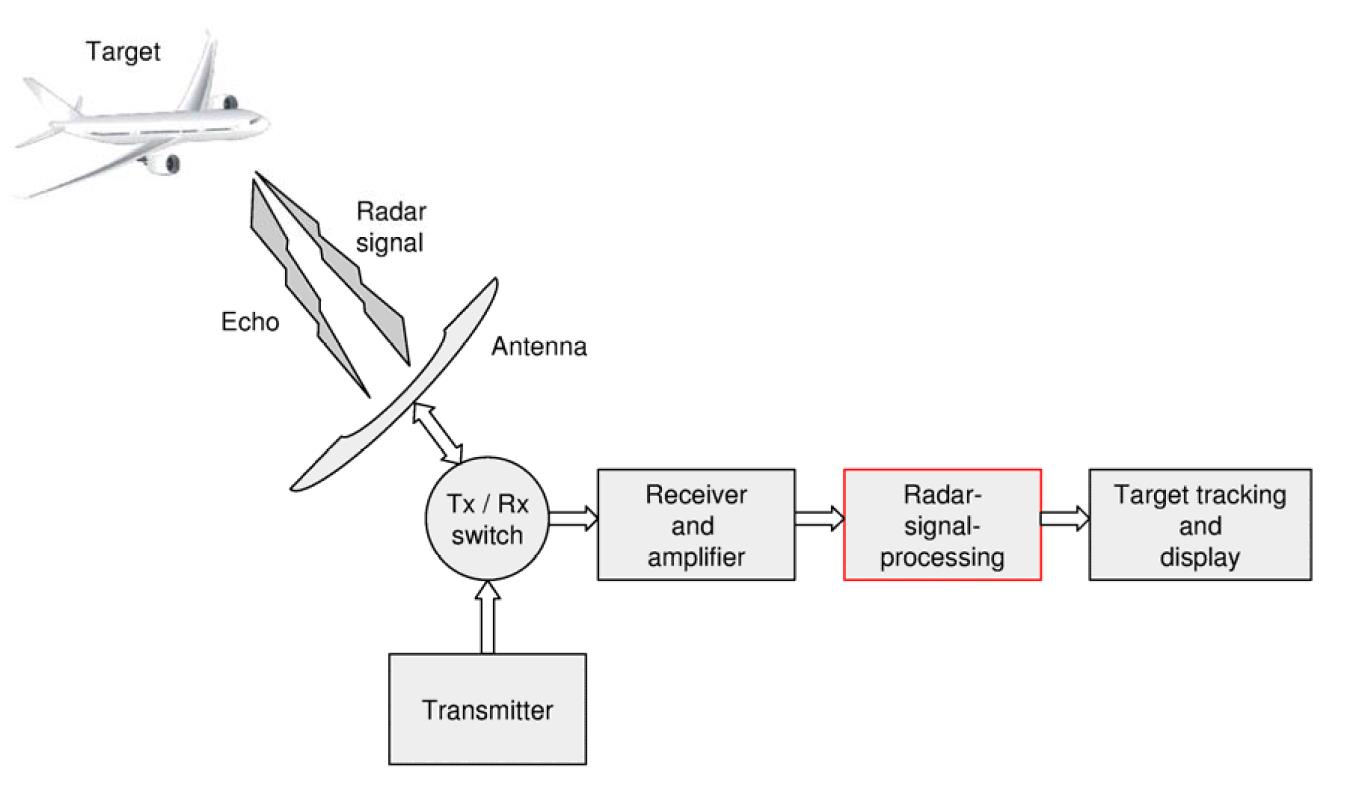
\includegraphics[width=130mm, height=75mm]{figures/radar_principle}
	\caption{Block Diagram of Pulse Doppler Radar \cite{Ludl}}
	\label{fig:intro:radar:blockdia}
\end{figure}

The time delay between sending the pulse and receiving the echo reveals distance to the target. The frequency shift in the echo tells the radial velocity of the target.
\begin{figure}[h!]
	\centering
	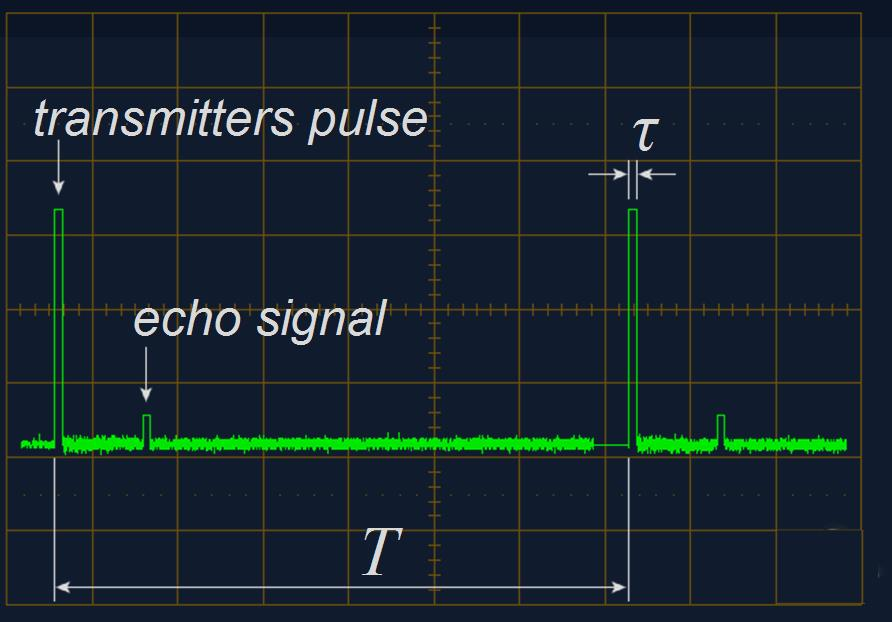
\includegraphics[width=75mm]{figures/trRx}
	\caption{Transmitter's Pulse and Echo Signal from Target \cite{radarTut}}
	\label{fig:intro:radar:txrx}
\end{figure}

Conventional waveband format is followed by manufacturers to address the radar operating frequency. Nowadays, radars are operated from 300MHz to 100GHz in different wavebands. The purpose and installation location of the radar determines the waveband. The accuracy of the radar is proportional to the operating frequency. Also, high frequency signals are more attenuated to water droplets and water vapours in the atmosphere. On the other hand, attenuation of the lower frequency signals is lower than high frequency signals. The typical use case of low frequency radar is in Early Warning Systems whereas high frequency radars are deployed in missile guidance systems \cite{radarExample}.

\subsection{Terminologies}
Radar systems use the spherical coordinate system to localize an object in the sky. The three following information are required to pin point an object relative to the Radar's position.

\textsl{\textbf{Azimuth angle ($\theta _{az}$):}} It is the angle between north and the target in horizontal plane. Azimuth angle can say whether the target is in the left side or right side to the north.

\textsl{\textbf{Elevation angle ($\varphi _{el}$):}} It is the angle between the target and Radar's local plane. Elevation says altitude of the target relative to the Radar. The Azimuth angle and Elevation angle of the Sun are explained in Figure \ref{fig:intro:radar:aziele}.

\textsl{\textbf{Radial distance (r):}} Distance between the target and Radar.\\

\begin{figure}[h!]
	\centering
	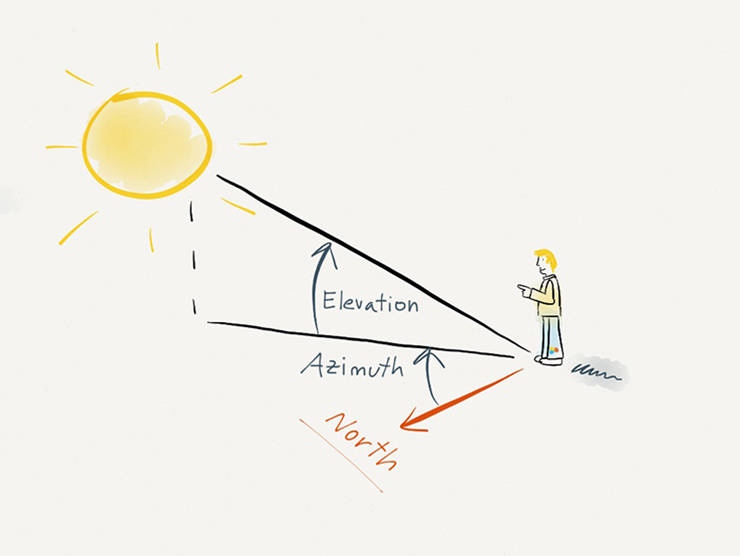
\includegraphics[width=75mm]{figures/azimuth_elevation}
	\caption{Azimuth and Elevation of the Sun \cite{aziEle}}
	\label{fig:intro:radar:aziele}
\end{figure}
\noindent
Other terminologies related to this thesis are explained here. \\[0.4cm]
\textsl{\textbf{Pulse:}} The Radar transmits an electromagnetic signal for a short duration (T$_{on}$) called pulse, then a break (T$_{off}$) follows to receive the echo of the pulse. This T$_{on}$ and T$_{off}$ together is called Pulse Repetition Time (PRT). Actual frequency of the electromagnetic wave transmitted during T$_{on}$ period is called carrier frequency.\\[0.2cm]
%\vspace*{0.2cm}
\noindent
\textsl{\textbf{Burst:}} The Radar sends $n$ number of pulses and listens to the echo signal. The combination of selected PRT and the number of pulses are called Burst. Figure \ref{fig:intro:radar:prf} shows two different bursts having 3 pulse count each.

\begin{figure}[h!]
	\centering
	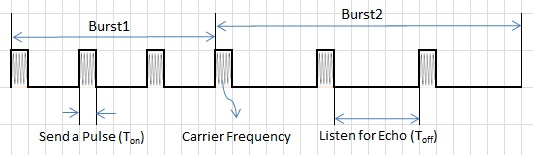
\includegraphics[]{figures/prf}
	\caption{Example of Burst}
	\label{fig:intro:radar:prf}
\end{figure}
\vspace*{0.2cm}
\noindent
\textsl{\textbf{PRF:}} Inverse of Pulse Repetition Time is called Pulse Repetition Frequency. \\
\noindent
\textsl{\textbf{Dwell:}} Group of 8 different bursts form a dwell.
\FloatBarrier

%%%%%%%%%%%%%%%%%%%%%%%%%%%%%%%%%%%%%
%%%%%%%%%%%%%%%%%%%%%%%%%%%%%%%%%%%%%
%%%%%%%%%%%%   SECTION   %%%%%%%%%%%%
%%%%%%%%%%%%%%%%%%%%%%%%%%%%%%%%%%%%%
%%%%%%%%%%%%%%%%%%%%%%%%%%%%%%%%%%%%%
\section{Motivation}
\label{sec:intro:motivation}
Radar is one of the core components of a combat air system. Range and accuracy of the Radar is important for missile system, guidance system, early warning system etc. Medium range (40nm) Radars are considered as suitable candidates to adopt low cost, compact ARM processors. They do not need several TFLOP of processing power to adhere to the requirements. The replaced Radar processor should be able to process Air to Air (A/A) Mode data and Air to Ground Mode (SAR) data. As a safety critical software, it should stick to the industrial standards DO-178B/C, ARINC-653 which have impact on design decisions.

The Radar modes shall be mapped to an Integrated Modular Avionics (IMA) processor and the following assessments are carried out. 
\begin{itemize}
	\itemsep0em
	\item Resulting processing latency
	\item Memory transfer bandwidth
	\item Memory utilization 
	\item CPU utilization
\end{itemize}

\noindent
Mode mapping activity covers the definition of 
\begin{itemize}
	\itemsep0em
	\item Mode allocation 
	\item Task allocation 
	\item Data distribution
	\item Communication schemes
\end{itemize}
\noindent
Results and possible improvements are discussed for further optimization.

%%%%%%%%%%%%%%%%%%%%%%%%%%%%%%%%%%%%%
%%%%%%%%%%%%%%%%%%%%%%%%%%%%%%%%%%%%%
%%%%%%%%%%%%   SECTION   %%%%%%%%%%%%
%%%%%%%%%%%%%%%%%%%%%%%%%%%%%%%%%%%%%
%%%%%%%%%%%%%%%%%%%%%%%%%%%%%%%%%%%%%
\section{Problem Statement}
\label{sec:intro:probstatement}
The Airborne Radar is subjected to operate on different Pulse Repetition Frequencies (PRF) to resolve ambiguity in distance and velocity. In the examined Radar application, it is fixed that 8 different bursts form a dwell. That is on every time the Radar scans a complete azimuth, several dwells are transmitted, echoes are received and analysed. The resulting worst case latency of the existing analysis is 15x dwell time (see Table \ref{tbl:mm:scheme1_true_latency}).  A typical dwell time is 54ms. An Eurofighter Typhoon moving at a speed of Mach 2 would move a distnace of 560 meters during this latency time. Half a kilometer difference between detection and display is very high for a typical Airborne Radar processor. \\

The acceptable latency range is maximum 2x dwell time. Since the system is in the early stage of development and to allow room for further requirements, the CPU utilization shall not exceed 50\%. The same is applicable for memory utilization and memory transfer bandwidth. The investigation of this thesis is to determine the number of processors required, mode mapping, data distribution, resulting processing latency and exploit the parallelism to achieve best result.

%%%%%%%%%%%%%%%%%%%%%%%%%%%%%%%%%%%%%
%%%%%%%%%%%%%%%%%%%%%%%%%%%%%%%%%%%%%
%%%%%%%%%%%%   SECTION   %%%%%%%%%%%%
%%%%%%%%%%%%%%%%%%%%%%%%%%%%%%%%%%%%%
%%%%%%%%%%%%%%%%%%%%%%%%%%%%%%%%%%%%%
\section{Contributions}
\label{sec:intro:contrib}
Benchmarks of the performance critical radar functions were given as inputs. They were meant for single core processors and thus single-threaded. One of the major works of this thesis is extending the benchmark program to replicate the Radar application, targeted for multicore and multi-threaded application.
In summary, the main contributions of this thesis are:

\begin{itemize}
\item{\bf Multicore Performance}
  \begin{itemize}
    \item Scalability and performance of the application on multicore environment are estimated. Shared resources, resource contention, race condition are considered.
    \item All the threads are set to execute the benchmarks simultaneously to ensure the maximum memory transfer bandwidth.
  \end{itemize}
\item {\bf Mode Mapping}
 	\begin{itemize}
 	\item Data dependencies are identified and evaluated by executing them in parallel using POSIX Threads.
   	\item Constrains on non-thread-safe benchmarks are discovered.
   	\item Optimal mode mapping schemes are proposed and their results are assessed.
	\end{itemize}
\item {\bf Measurement Tools}
  \begin{itemize}
      \item Developed automated scripts to measure peak memory utilization, CPU load, memory transfer bandwidth and processing latency.
      \item Worst case execution time is computed by measuring the maximum execution time of 1000 runs.
  \end{itemize}
 \item {\bf Verification of Results}
   \begin{itemize}
       \item Results of multicore application are verified against the single core application.
   \end{itemize}
\end{itemize}

%%%%%%%%%%%%%%%%%%%%%%%%%%%%%%%%%%%%%
%%%%%%%%%%%%%%%%%%%%%%%%%%%%%%%%%%%%%
%%%%%%%%%%%%   SECTION   %%%%%%%%%%%%
%%%%%%%%%%%%%%%%%%%%%%%%%%%%%%%%%%%%%
%%%%%%%%%%%%%%%%%%%%%%%%%%%%%%%%%%%%%
\section{Thesis Outline}
\label{sec:intro:outline}

The rest of this thesis is organized as follows:

%\begin{compactitem}
\begin{itemize}
	\item \textbf{Chapter \ref{chap:bg_related_work}:} Explains about IMA architecture, experimental setup and related work concerning ARM processors in Radar application.

	\item \textbf{Chapter \ref{chap:existing_analysis}:} Discusses results of the existing analysis done by Airbus Defence and Space GmbH.

	\item \textbf{Chapter \ref{chap:testbed}} Explains pros and cons of the existing analysis, test bed information and important design choices.

	\item \textbf{Chapter \ref{chap:mode_mapping}:}  Proposes new schemes of mode mapping and verifies their correctness via implementation. Results of the new schemes are analysed.

	\item \textbf{Chapter \ref{chap:conclusion}:} Summarizes this thesis with a conclusion and proposes future work regarding the new analysis.
\end{itemize}
%

